\newcommand{\onelinerule}{\rule[2.3ex]{0pt}{0pt}}
\newcommand{\twolinerule}{\rule[6.2ex]{0pt}{0pt}}
\newcommand{\respuesta}{\framebox[\textwidth]{\twolinerule}}
\newcommand{\nombre}{%
  \begin{tikzpicture}[xscale=.4,yscale=.7]
    \draw (0, 0) rectangle (22, 1);
  \end{tikzpicture}%
}
%\newcommand{\rol}   {\framebox[0.3\textwidth]{\onelinerule}}
\newcommand{\rol}{%
  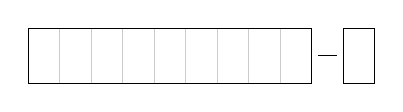
\begin{tikzpicture}[xscale=.4,yscale=.7]
    \draw[gray!40] ( 0, 0) grid      ( 9, 1);
    \draw          ( 0, 0) rectangle ( 9, 1);
    \draw          (10, 0) rectangle (11, 1);
    \draw (9 + .2, .5) -- (10 - .2, .5);
  \end{tikzpicture}%
}
\newcommand{\li}{\lstinline}
\providecommand{\pond}[1]{[{\small\textbf{#1\%}}]}

\lstdefinelanguage{py}{%
  classoffset=0,%
    morekeywords={%
      False,class,finally,is,return,None,continue,for,lambda,try,%
      True,def,from,nonlocal,while,and,del,global,not,with,print,%
      as,elif,if,or,yield,assert,else,import,pass,break,except,in,raise},%
    keywordstyle=\color{black!80}\bfseries,%
  classoffset=1,
    morekeywords={int,float,str,abs,len,raw_input,exit,range,min,max,%
      set,dict,tuple,list,bool,complex,round,sum,all,any,zip,map,filter,%
      sorted,reversed,dir,file,frozenset,open,%
      array,zeros,ones,arange,linspace,eye,diag,dot},
    keywordstyle=\color{black!50}\bfseries,%
  classoffset=0,%
  sensitive=true,%
  morecomment=[l]\#,%
  morestring=[b]',%
  morestring=[b]",%
  stringstyle=\em,%
}

\lstdefinelanguage{testcase}{%
  moredelim=[is][\bfseries]{`}{`},%
  backgroundcolor=\color{gray!20},%
}

\lstdefinelanguage{file}{%
  frame=single,%
}

\lstset{language=py}
\lstset{basicstyle=\ttfamily}
\lstset{columns=fixed}
\lstset{upquote=true}
\lstset{showstringspaces=false}
\lstset{rangeprefix=\#\ }
\lstset{includerangemarker=false}

\newlist{certamen}{enumerate}{1}
\setlist[certamen]{%
  label=\arabic*.,
  font=\LARGE\bfseries,%
  labelindent=-.5in,%
  leftmargin=0pt,%
  labelsep=1em%
}

